\section{Refactor}
\subsection{How it was}
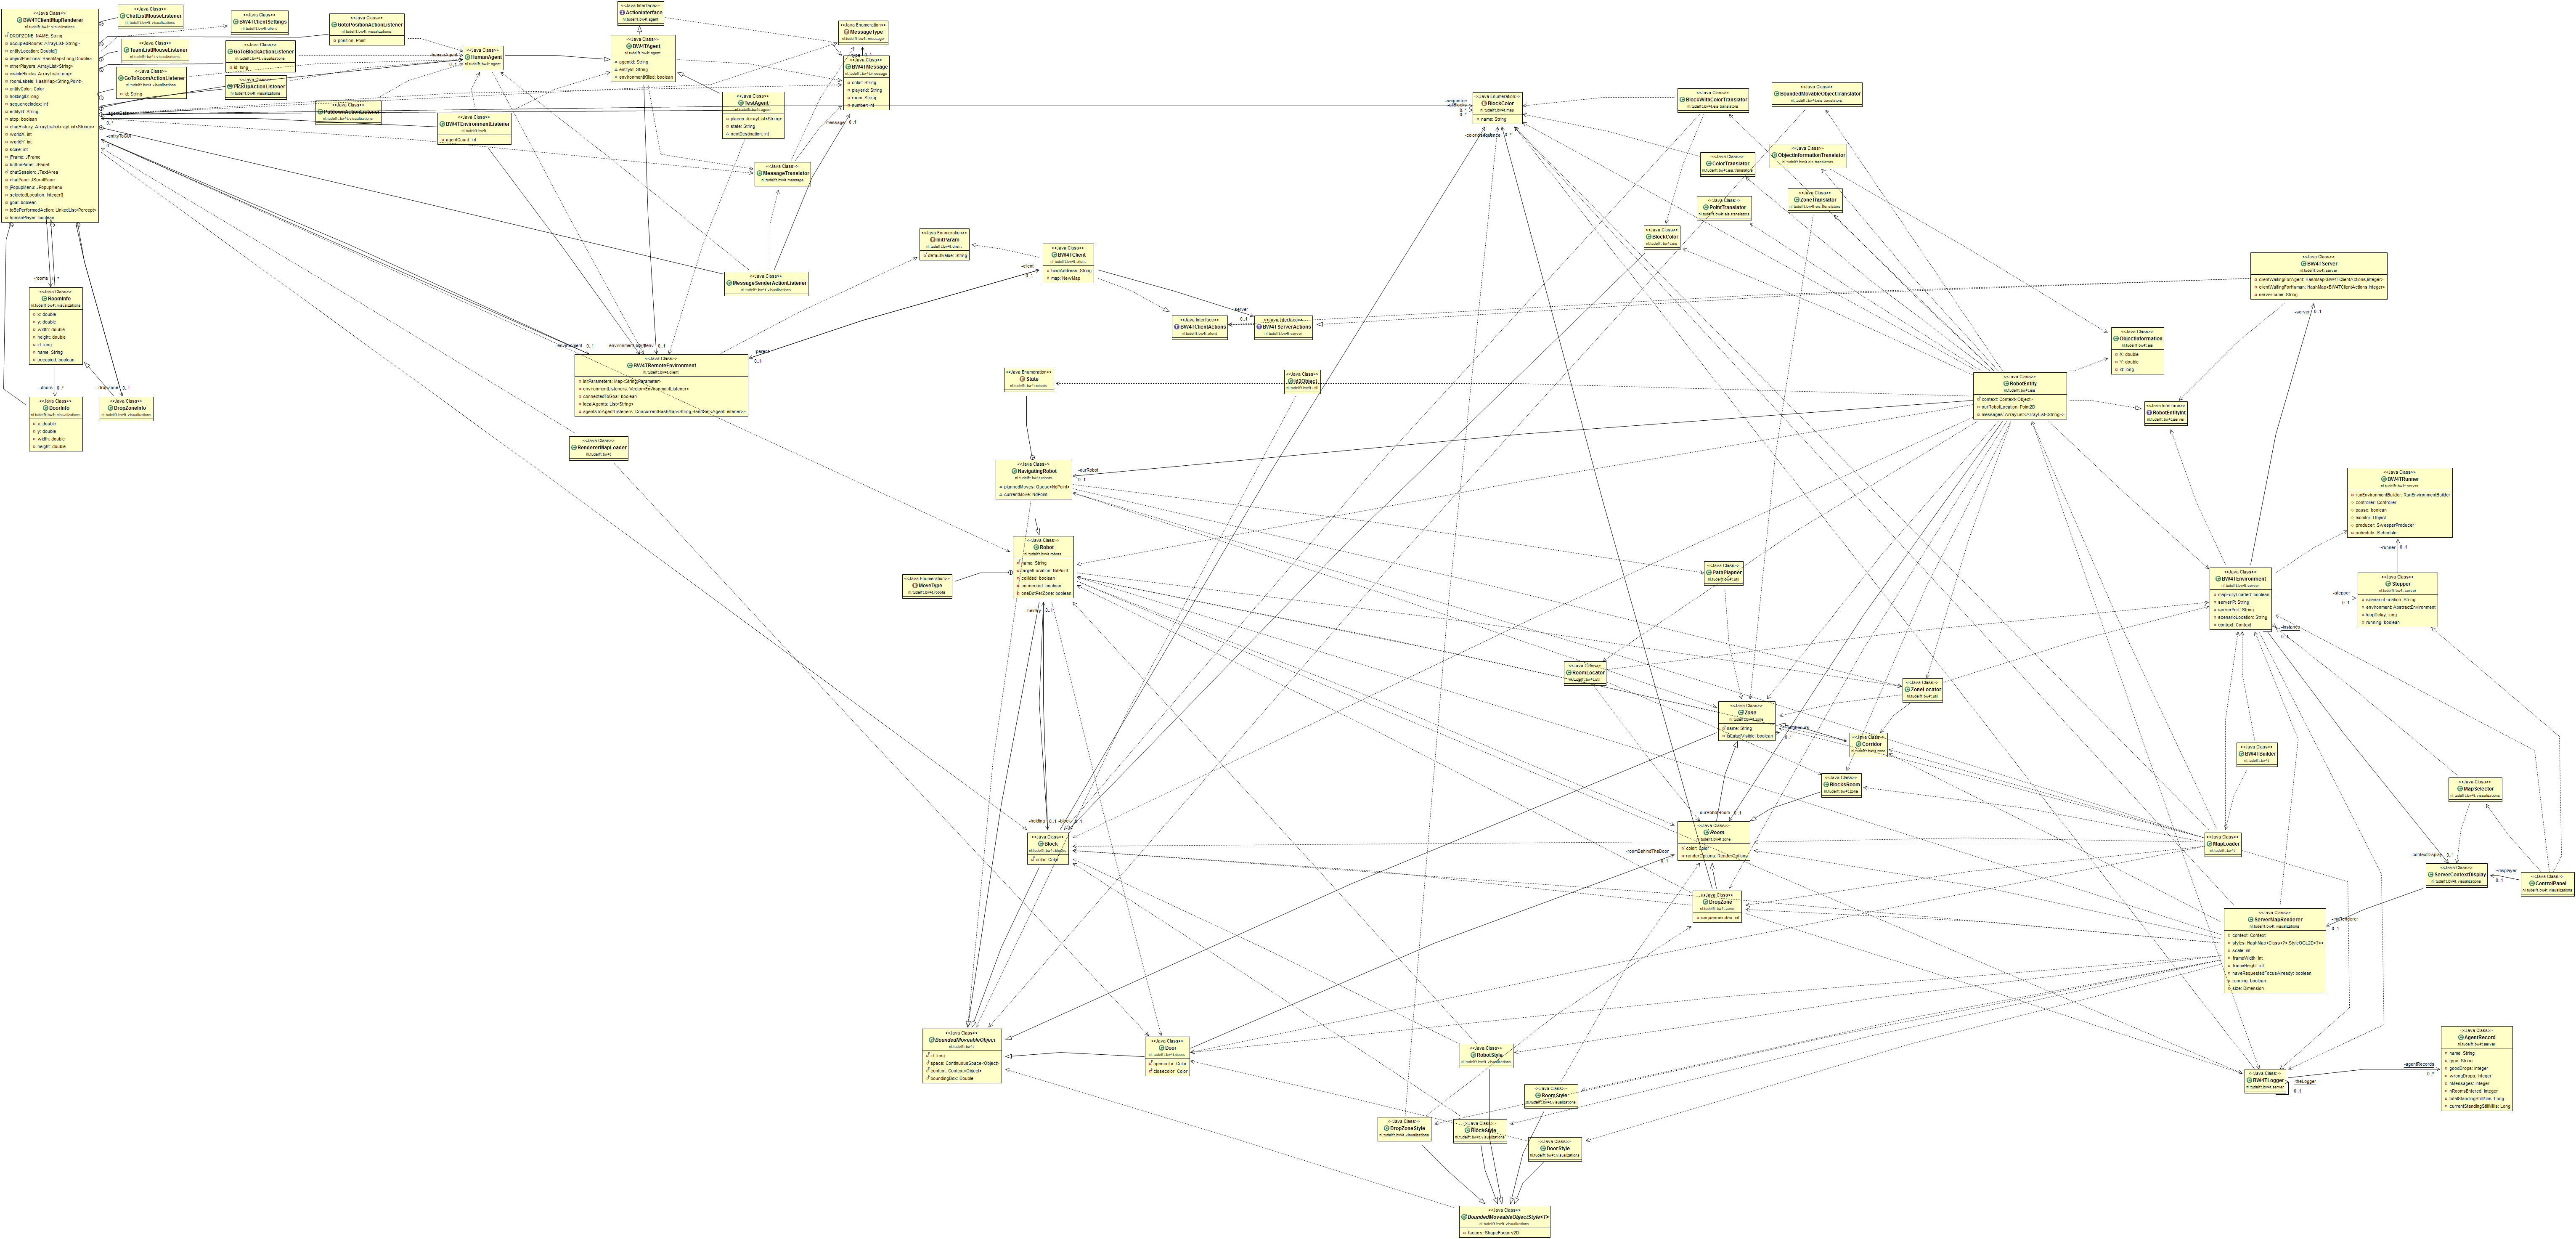
\includegraphics[width=\linewidth]{Transferability/old.png}
As can be seen in the UML diagram above, many classes were connected, Documentation was inadequate and no tests were written. These factors made it very hard for us to understand and debug the code base.
It took quite some time to find out what a piece of code exactly did, what function a method had, what the difference between methods and classes was and what the connection between pieces of code was.
After some weeks of exploring the code base and the UML diagrams belonging to the code base, we found out that there was no clear structure at all. There was a client and a server, but all communication went through the BW4TEnvironment class. So the first thing we did, was deciding how to split up the code, such that we got a clear Client-Server Architecture. \\
\indent Take a look at the attachments as well for some examples of the old code.
In the old system, Repast was used. Problem was that many functions in Repast were custom written as well and the entire Repast package needed to be installed. This caused the system to grow very large (500 MB for Repast only).

\subsection{What we achieved}
Server \\
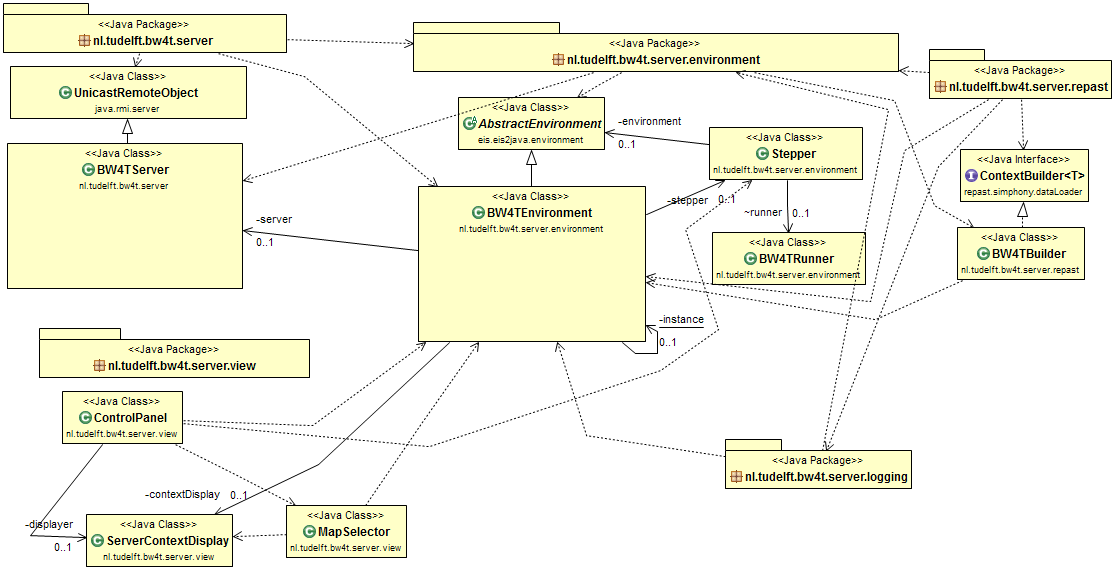
\includegraphics[width=\linewidth]{Transferability/server_simplified_boxed.png}
\\ Client \\
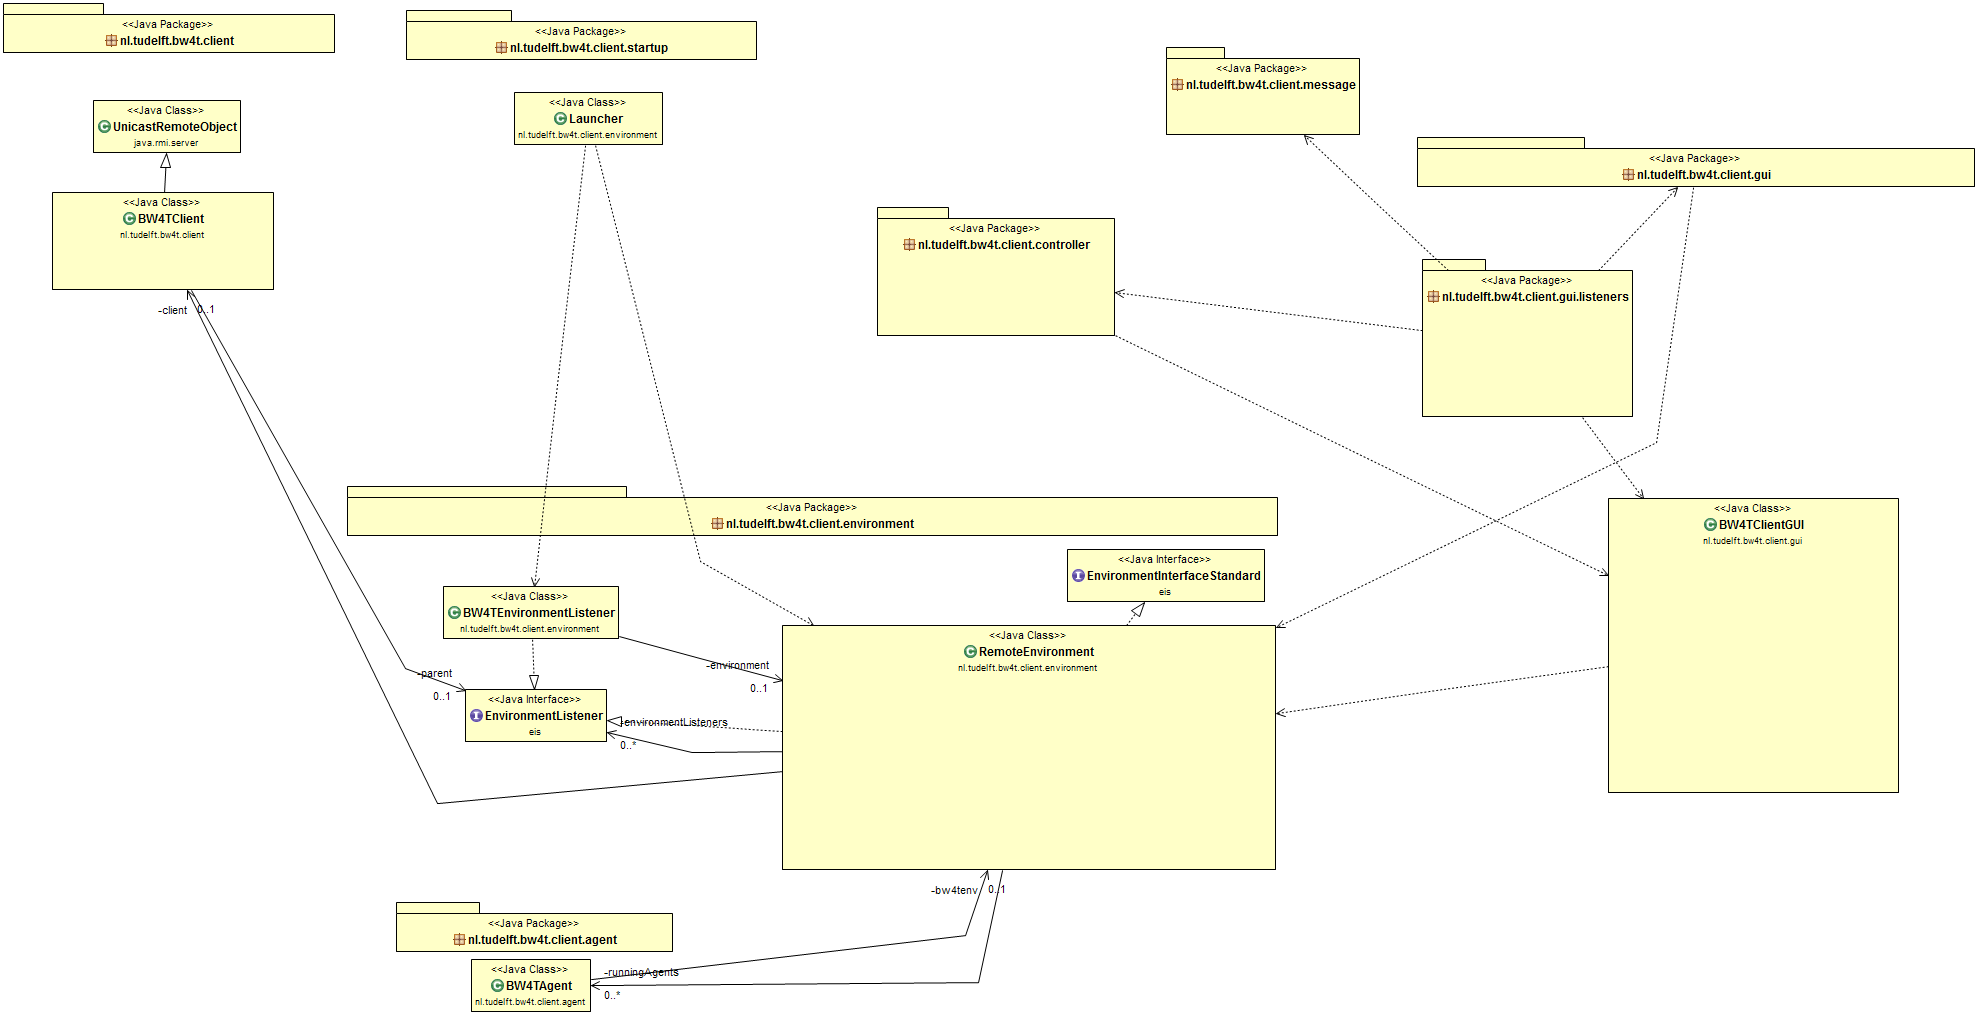
\includegraphics[width=\linewidth]{Transferability/client_simplified_boxed.png}
The customer wanted a clear structure to be added to the code base. Besides that, the code had to be rewritten so that it would be easier to adjust and maintain the code. Adding new features should than automatically become easier as well. \\
\indent We decided to put classes which the client needs and the server does not need into the client package. This does not cause any errors in the server, and anything needed by the client is present. Afterward, we did the same for the server. All classes needed by the server and not by the client are put in the server package. The classes that are needed by both, we put in the core package. The core can be seen as a library, it can be used by both the server and the client when needed. For the client and the server, simplified diagrams are shown above.
We chose to use Maven as an outline for the project, because Maven has a perfect way of handling those parts and the dependencies between them. Other dependencies such as EIS and Repast can be put in the resources folder and Maven takes care of the rest. \\
\indent After everything was set up, we took a deeper look at the code. Trying to figure out what could be replaced by Repast was a big task that, for now, unfortunately led to nothing. Repast is a big bunch of interfaces which can guide your simulation of agents. Unfortunately, there were some problems with the connection to GOAL. GOAL can be paused and resumed whenever the user wants to, but Repast will continue to run, which will lead to false simulations and results. However because we only had 5 weeks to refactor the entire code base, we decided to leave Repast as it is for now. The chance of breaking the project was too big, as we had to deliver a fully working product in only 5 weeks. \\
\indent But we did manage to get the Repast functions more efficient. In combination with Maven, we pulled Repast apart and only added the dependencies that are really needed. Now the Repast functionality used is only 8 MB. Besides that, we made sure the newest version of Repast is used.
So we started looking at what could be refactored. We created our own UML class diagram, and got really shocked about all connections and tried to figure out what the god classes are and how we could make them smaller. We immediately saw that BW4TRemoteEnvironment was the hugest class in the project, so that had to be refactored. BW4TClientMapRenderer was the second god class we handled. We tried to pick pieces of code that belong together and diffused it to a different class. \\
\indent Then we found the custom BW4TLogger, a logger implemented to print anything the bot does. We thought that it would be very practical to export the logging to Log4j (an apache library). Now two kinds of logs are made, one kind that prints all the bot's actions to the log file and the other prints the debug issues in the code to the console. Now it can easily be adapted, if anything new from a bot is wanting to be logged, you just log it to BOTLOG level and it appears in the log file.

\subsection{Attachments} 
This section contains some examples of the old code base that we found. It were examples of what we wanted to adjust and make sure it never happens again.

Empty methods.\\
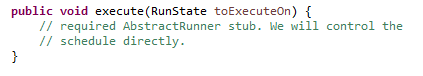
\includegraphics[width=\linewidth]{Transferability/emptyMethod.PNG} \\ 

Two methods that look alike, but the difference is nowhere to be found .\\
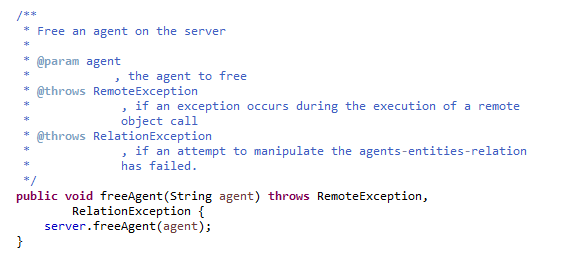
\includegraphics[width=\linewidth]{Transferability/freeAgentNoClue.PNG}
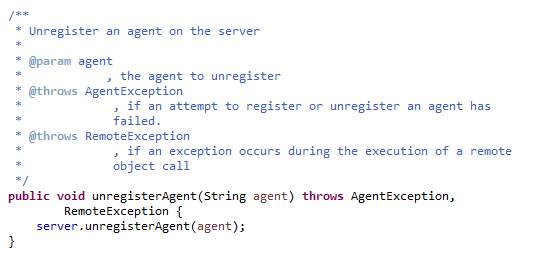
\includegraphics[width=\linewidth]{Transferability/unregisterAgentNoClue.PNG} \\ 

Hacks \\
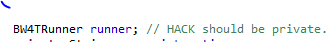
\includegraphics[width=\linewidth]{Transferability/HackWTF.PNG} \\ 

Commented code.\\
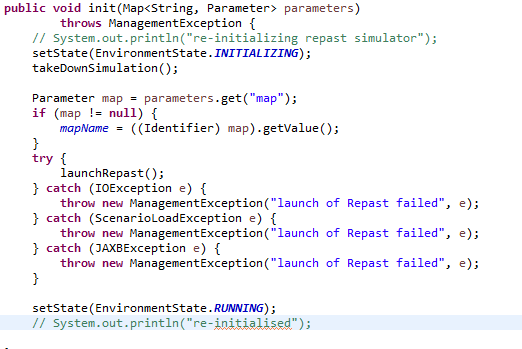
\includegraphics[width=\linewidth]{Transferability/lelijkCode.PNG} \\ 

No checks whether code satisfies pre condition.\\
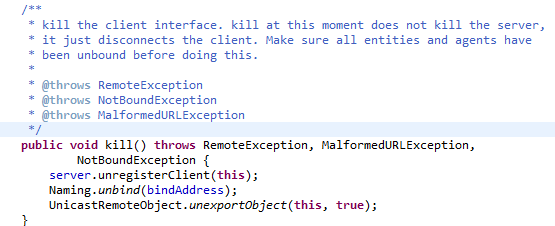
\includegraphics[width=\linewidth]{Transferability/noEntityCheck.PNG} \\ 

Nothing tested, everything is assumed to work.\\
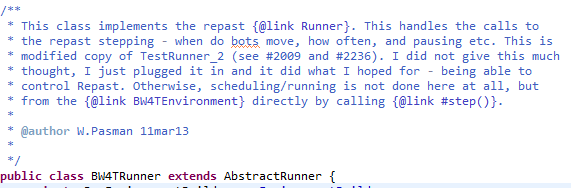
\includegraphics[width=\linewidth]{Transferability/notTested.PNG} \\ 

TODO's and should-be-fixed's.\\
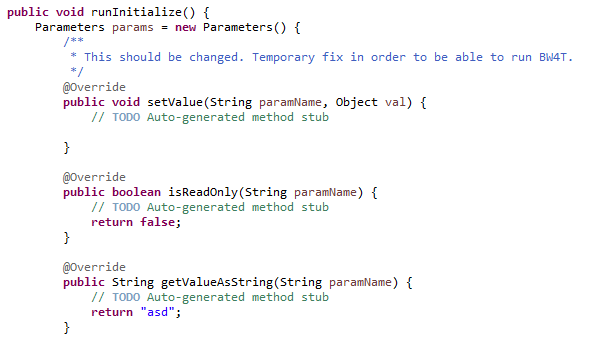
\includegraphics[width=\linewidth]{Transferability/TODOs+shouldBeFixed.PNG} \\